\documentclass{amia}
\usepackage{graphicx}
\usepackage[labelfont=bf]{caption}
\usepackage[superscript,nomove]{cite}
\usepackage{color}
\usepackage{multirow}
\renewcommand*{\thefootnote}{\alph{footnote}}

\begin{document}

\title{Machine Learning Methods for Discourse Segmentation of Communications in E-Mail Based Behavioral Interventions}

\author{Mehedi Hasan, BS$^{1}$\footnote{Authors provided an equal contribution. \label{footnote1}}, Alexander Kotov, PhD$^{1}$\textsuperscript{\ref{footnote1}}, Sylvie Naar, PhD$^{2}$, Gwen L. Alexander, PhD$^{3}$, April Idalski Carcone, PhD$^{4}$}

\institutes{
$^1$Department of Computer Science, Wayne State University, Detroit, Michigan \\  
$^2$Center for Translational Behavioral Research, Department of Behavioral Sciences and Social Medicine, Florida State University, Tallahassee, Florida\\
$^3$Department of Public Health Sciences, Henry Ford Health System, Detroit, Michigan\\
$^4$Department of Family Medicine and Public Health Sciences, School of Medicine, Wayne State University, Detroit, Michigan\\
}

\maketitle

\noindent{\bf Abstract}
\textit{Communication science approaches to developing effective behavior interventions, such as motivational interviewing (MI), are limited by the traditionally manual qualitative coding of communication exchanges, which is a very resource-intensive and time-consuming process. This study focuses on the analysis of e-Coaching sessions, behavior interventions that are delivered via email and grounded in the principles of MI. A critical step towards automated annotation of e-Coaching communication exchanges is segmentation of emails into textual fragments that correspond to MI behaviors. In this work, we formulate this task as a classification problem and propose word embeddings, punctuation and part-of-speech features to address it. We experimented both with traditional machine learning method, conditional random fields (CRF) and deep learning methods, such as multilayer perceptrons (MLP), bidirectional recurrent neural networks (BRNN) and convolutional recurrent neural networks (CRNN). Results indicate that CRNN outperformed CRF, MLP and BRNN achieving 0.989 macro F1-score overall and 0.825 macro F1-score for detecting new segment.}

\section*{Introduction}
The emergence of e-Health technologies opened up new ways to deliver a variety of behavioral interventions to any demographic group of patients in any geographical location. Motivational interviewing (MI), an evidence-based communication technique to increase intrinsic motivation and self-efficacy for behavior change,\cite{miller2012motivational,miller2009toward} is one type of these interventions. MI sessions are generally aimed at eliciting ``change talk'', or statements of intrinsic motivation about patients' own desire, ability, reasons, need for and commitment to behavior change, which have been established by previous research\cite{apodaca2009mechanisms} as a reliable mediator of health behavior change. However, communication science approaches to understanding the efficacy of MI are inherently limited by traditional qualitative coding methods. 

Qualitative coding of motivational interviews with pre-defined codes has been traditionally performed manually by trained annotators, which is a tedious and resource-intensive process that involves several iterations of reading, comprehension and interpretation of interview transcripts. Rapidly developing computational technologies, specifically, machine learning methods, offer a unique opportunity to accelerate this process. In particular, machine learning methods have been successfully applied to a variety of analytical tasks involving textual data, such as classification\cite{nigam2000text} and sentiment analysis.\cite{wang2012baselines} In our previous work, we examined the utility of machine learning methods for automated annotation \cite{hasan2016study,kotov2015interpretable} and analysis \cite{hasan2018predicting} of in-person MI sessions. Specifically, we demonstrated that machine learning methods can be utilized for annotation of MI transcripts according to a simple communication code scheme with the accuracy comparable to human coders.\cite{hasan2016study} Experimental data utilized in these studies, however, were prepared by transcribing audio conversations, which were clearly segmented into utterances by a counselor, a patient and a caregiver. 

In this study, we focus on the analysis of e-Coaching sessions, behavior interventions that are delivered via email and grounded in the principles of motivational interviewing. Specifically, the e-Coaches involved in this study used emails to communicate motivation-enhancing messages that encourage healthy eating among GenY adolescents. E-coaching data is comprised of email responses, which are free-text documents, unlike more traditional dyadic clinical interviews that are naturally segmented into utterances due to their conversational nature.

The unstructured nature of e-Coaching exchanges poses a unique set of challenges for their qualitative analysis. Usually, email segments are automatically coded with the Minority Youth-Sequential Coding of Process Exchanges (MYSCOPE), \cite{carcone2013provider} a qualitative coding scheme to characterize patient-coach communication during email exchanges. A significant barrier to fully automating the behavior coding process of e-Coaching emails is their segmentation into textual fragments that correspond to distinct communication behaviors. Automating this task is a unique and challenging problem due to the following major reasons:

\begin{enumerate}
\item Emails are unstructured text that contains informal information exchange in a non-traditional format. For example, an e-Coach usually responds to several queries of a patient in one email. However, a provider utterance of MI transcript denotes a particular response for a query of a patient during a traditional MI interview session, which involve a dialogue between a provider and a patient. 
\item Discourse segments in e-Coaching emails do not necessarily correspond to sentences or collection of sentences. One sentence can be segmented into multiple MI behavior fragments. On the other hand, an MI behavior may comprise several sentences.
\end{enumerate}

Figure~\ref{fig:text-segment} illustrates a segmentation of an e-Coaching email exchange, in which the first sentence is segmented into 2 MI behavior fragments, while the fourth and fifth segments correspond to one and three sentences, respectively. Segmentation of e-Coaching emails corresponds to a special type of discourse analysis \cite{webber2012discourse} aimed at better understanding the effective e-Coaching communication strategies and revealing the unique socio-psychological characteristics of a patient.

\begin{figure}[!htb]
    \centering
    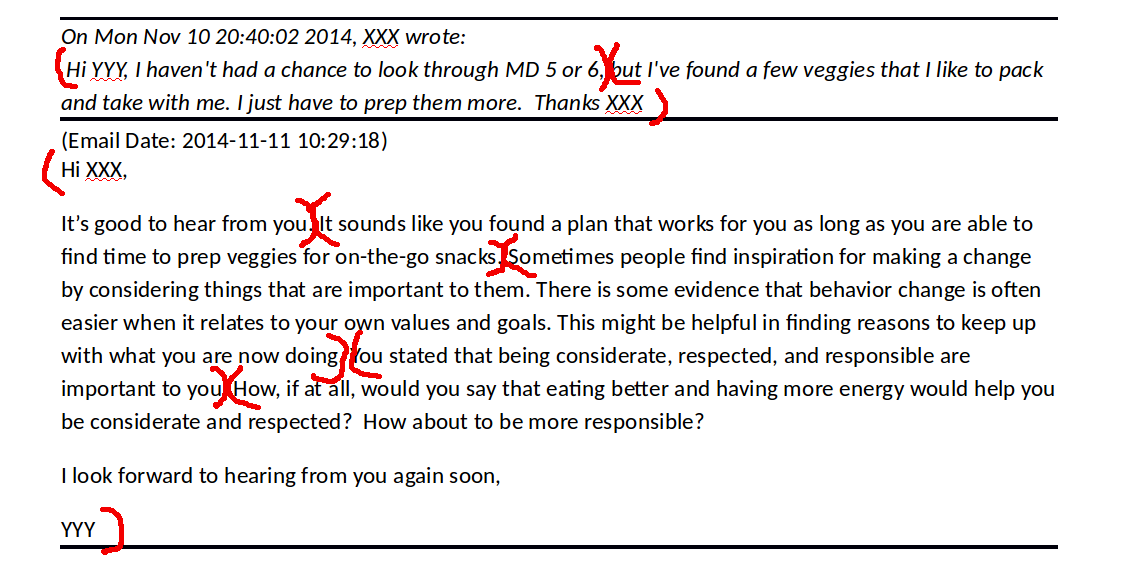
\includegraphics[width=0.7\textwidth]{figures/segment-example.png}
    \caption{\textbf{Example of e-Coaching emails segmented into fragments that correspond to MI behaviors of an e-Coach and a patient}}
    \label{fig:text-segment}
\end{figure}

Recently, an online clinical intervention called MENU GenY (Making Effective Nutrition Choices for Generation Y) was proposed and evaluated. \cite{alexander2017motivations} MENU GenY is a technology-based public health intervention that relies on personalized e-coaching to encourage increased fruit and vegetable intake among young adults, aged 21-30. The goal of MENU GenY was to develop a better coding dictionary among GenY to improve eating habits. However, segmentation of clinical exchange in the context of electronically delivered interventions, in particular, segmentation of clinical interaction text into groups of MI behaviors, is still performed manually, which slows down qualitative analysis of these interventions. This study proposes several machine learning methods to address this problem and the authors are unaware of any other work that focused on the same problem.

The goal of this research study is to assess the applicability of machine learning methods for automated segmentation of e-Coaching emails into textual fragments corresponding to individual behaviors, which is the first step of the coding process of e-Coaching communications. In particular, we introduced word embeddings or lexical, punctuation and  part-of-speech (POS) features and experimented with both traditional supervised machine learning method, linear-chain conditional random fields (CRF)\cite{lafferty2001conditional} and deep learning methods, such as multilayer perceptrons (MLP),\cite{rumelhart1986learning} bidirectional recurrent neural networks (BRNN)\cite{schuster1997bidirectional} and convolutional recurrent neural networks (CRNN),\cite{treviso2017sentence} to find the best performing method and feature combination. 

Relevant previous work in the biomedical domain primarily focused on segmentation of text into sections and headers of electronic health records (EHR)\cite{apostolova2009automatic,denny2009evaluation,tepper2012statistical,cho2002text} or sentence boundary detection of EHR.\cite{griffis2016quantitative,kreuzthaler2015detection,treviso2017sentence} Apostolova et al. applied SVM along with word-vector cosine similarity metric combined with several heuristics to segment clinical reports in EHR into sections, such as demographics, history, procedure, finding and impression.\cite{apostolova2009automatic} After identification of each line in the document, Tepper et al. trained Maximum Entropy models to classify the document into pre-defined sections, such as general patient information, provider information, medical condition, medical history, clinical history, findings, impression, etc.\cite{tepper2012statistical} Denny et al. proposed a SecTag algorithm, which combined natural language processing techniques, terminology-based rules and a Naive Bayes classifier to identify the sections and headers that achieved 99\% recall with 95.6\% precision. \cite{denny2009evaluation} On the other hand, SVM based on prosodic and part of speech features \cite{kreuzthaler2015detection} and recurrent convolutional neural networks using word embeddings \cite{griffis2016quantitative} were utilized for detecting sentence boundaries in EHR. Liu et al. have shown that a linear chain CRF performed better than the hidden markov model and Maxent in sentence boundary detection, evaluated using the official
NIST evaluation tools.\cite{liu2005using} Recently, Treviso et al. proposed a recurrent convolutional neural network for automatic identification of sentence boundary in a neuropsychological text in the Portuguese language.\cite{treviso2017sentence} Their proposed model combined prosodic and part of speech features with pre-trained GloVe word embeddings,\cite{pennington2014glove} which achieved 0.74 F1-score in sentence boundary detection on the Brazilian constitution dataset. Segmentation of e-Coaching emails is different from a traditional shallow discourse analysis of conversations \cite{galley2003discourse} in that the focus is on segmentation, rather than on determining the types of transitions between the utterances or assigning utterances to speakers.

Our proposed approach is novel for the segmentation of e-Coaching emails since previous studies mainly focused on the segmentation of EHR documents into sections, headers and sentences. However, this study segmented clinical exchange into groups of MI behaviors which will significantly reduce the amount of resource and time required to segment clinical exchange manually. Furthermore, these segmentation models could be integrated with auto coding classifiers to build a software pipeline for automated annotation of clinical exchanges.
  
\section*{Methods}
\subsection*{\textit{Data collection}}

The experimental dataset for this work was constructed from 49 e-coaching sessions, which include a total of 3,138 segmented and annotated MI behaviors. Each session represents an MI intervention delivered via email. We formulate the segmentation task as a binary classification problem where each word or punctuation mark annotated with a label 1 or 0, to indicate whether it precedes a new segment or not. In total, we obtained 95,777 words and 7,140 punctuation marks, which include 3,138 ``new segment'' and 99,779 ``same segment'' instances. In this study, we experimented with traditional machine learning method, conditional random fields (CRF)\cite{lafferty2001conditional} and deep learning methods, such as multilayer perceptrons (MLP),\cite{rumelhart1986learning} bidirectional recurrent neural networks (bidirectional RNN or simply BRNN)\cite{schuster1997bidirectional} and convolutional recurrent neural networks (CRNN).\cite{treviso2017sentence} For MLP models, samples were created with $2l$ words or punctuations at each step in a word sequence, where a sample contains next $l$ words or punctuations and prior $l$ words or punctuations including current word or punctuation. Each sample is classified into either ``new segment'' or ``same segment'' based on whether the $l^{th}$ word or punctuation in the gold standard precedes a new segment or not. For CRF, BRNN and CRNN models, an email was taken as input sequence, such that POS tags and word embeddings of each word or punctuation mark were used as input and binary labels (1 or 0) corresponding to ``new segment'' and ``same segment'' classification decision were considered as the output of the model at each step. In the gold standard, words or punctuations within the same segment were assigned the label of 0 and the last word or punctuation mark of a segment were assigned the label of 1.     

\subsection*{\textit{Features}}

We utilized three types of features in conjunction with CRF, MLP, BRNN and CRNN methods: word embeddings or lexical features, punctuation and POS features. Since POS tags have been shown to be effective semantic abstractions of individual words, we used POS features for our experiment.\cite{liu2005using,treviso2017sentence} To extract our POS features, we tag the e-Coaching emails using the NLTK POS tagger. Punctuation marks, which correspond to one of the symbols \{`.', `,', `!', `?', `:', `;'\} between a pair of words, are also employed as a feature since punctuation marks designate the boundary of a sentence, clause and phrase and often also correspond to a segment boundary.\cite{cho2002text} For natural language processing (NLP) tasks, inputs are received as a text where words can be considered as the basic processing unit. Therefore, it is important to represent a word in such a way that it carries all relevant information. Word embeddings are one of this representation where each word represented as a real-valued vector in a high dimensional vector space. The distributed representation of word allows capturing semantic, syntactic and morphological information from large unannotated corpora.\cite{pennington2014glove, mikolov2013distributed} In our experiment, we utilized embeddings estimated on Google News corpus consisting of 1.6 billion words referred to pre-trained word2vec word embeddings.\footnote{https://code.google.com/p/word2vec/} When words or punctuation marks are not found in the pre-trained word vectors, we utilized word embeddings trained with our e-Coaching email corpus referred to trained word embeddings. CRF utilized lexical features which represent each word in an e-Coaching email. 

\subsection*{\textit{Classifiers}}

In the present study, we experimented with four different classifiers, including one traditional machine learning method, CRF and three deep learning models. Since deep learning methods provide a flexible architecture for constructing and synthesizing complex models, we take the advantage of this flexibility to test MLP, BRNN and CRNN models for the task of segmentation of e-Coaching emails.

\textbf{Conditional Random Fields}: CRF has been widely used in various NLP tasks including part-of-speech tagging and segmentation tasks.\cite{lafferty2001conditional, hirohata2008identifying} Unlike a maximum entropy Markov model which uses per-state exponential models for the conditional probabilities of next states given the current state, a CRF is modeled with an exponential distribution provides the conditional distribution of the entire output sequence given the observation sequence. A traditional linear-chain CRF model is defined as a conditional probability distribution $p(y|x)$ for output and input sequences, $y$ and $x$, by the Eq. \ref{Eq:crf}

\begin{equation}
\label{Eq:crf}
p(y|x) = \frac{1}{Z_x}\exp{\left(\sum_{t=1}^{T}\sum_{k}^{}\lambda_k f_k(y_{t-1}, y_t, x, t)\right)} \\
\end{equation}

Here $Z_x$ is a normalization factor over all possible labelings of $x$, and $f_k(y_{t-1}, y_t, x, t)$ is a feature function, and $\lambda_k$ is a learned weight associated with feature $f_k$. The optimal output sequence $y^*$ for an input sequence $x$, $y^* = {arg\,max}_y p(y|x)$, is obtained efficiently by the Viterbi algorithm. In our experiments, the following features were utilized with CRF models: i) current word or punctuation ii) next and previous 3 words or punctuations iii) binary feature indicating the word or punctuation is a special character (';', '?', '.', ',', '!', ':', etc) or not iv) binary feature indicating the word is a title word or not? (e.g. ``The'' is a title word but ``the'' is not) v) POS tags   

\textbf{Multilayer Perceptrons}: MLP is a feed-forward artificial neural network which maps set of input onto a set of appropriate output.\cite{rumelhart1986learning} Figure~\ref{fig:mlp} shows a multilayer perceptron with a single hidden layer. In MLP networks, there is no cycles or loops and information moves forward only, from the input nodes through the hidden nodes and to the output nodes. This study utilized MLP with a nonlinear activation function (relu) and one hidden layer consisting of 128 hidden units. In order to prevent over-fitting, we implement dropout on fully connected layers, which randomly hide some neurons during the training phase. \cite{srivastava2014dropout} Dropout is also applied to the fully connected layers in BRNN and CRNN models. 

\begin{figure}[!htb]
    \centering
    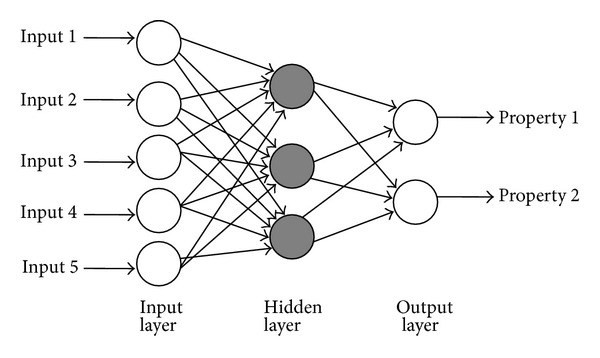
\includegraphics[width=0.5\textwidth]{figures/mlp.jpeg}
    \caption{\textbf{A multi layer perceptron with a single hidden layer}}
    \label{fig:mlp}
\end{figure}

\textbf{Bidirectional Recurrent Neural Networks}: BRNN is a neural network designed to capture sequential patterns by considering both past \& future inputs as well as complex relationships between input features and output labels.\cite{schuster1997bidirectional} The output of BRNN layer is computed with the summation of the forward RNN output and backward RNN output. Gated Recurrent Units (GRU)\cite{chung2014empirical} are utilized as RNNs that are capable of handling variable size input sequence and have an internal memory that can be reset. Figure~\ref{fig:crnn} will represent an architecture of BRNN if convolution layer is removed.  

\textbf{Convolutional Recurrent Neural Networks}: CRNN is a deep neural networks architecture,\cite{treviso2017sentence} shown in Figure~\ref{fig:crnn}, consisting of 5 layers: 1) input layer 2) embedding layer 3) convolution layer with max pooling 4) BRNN layer 5) fully connected layer with dropout and sigmoid output. 

\begin{figure}[!htb]
    \centering
    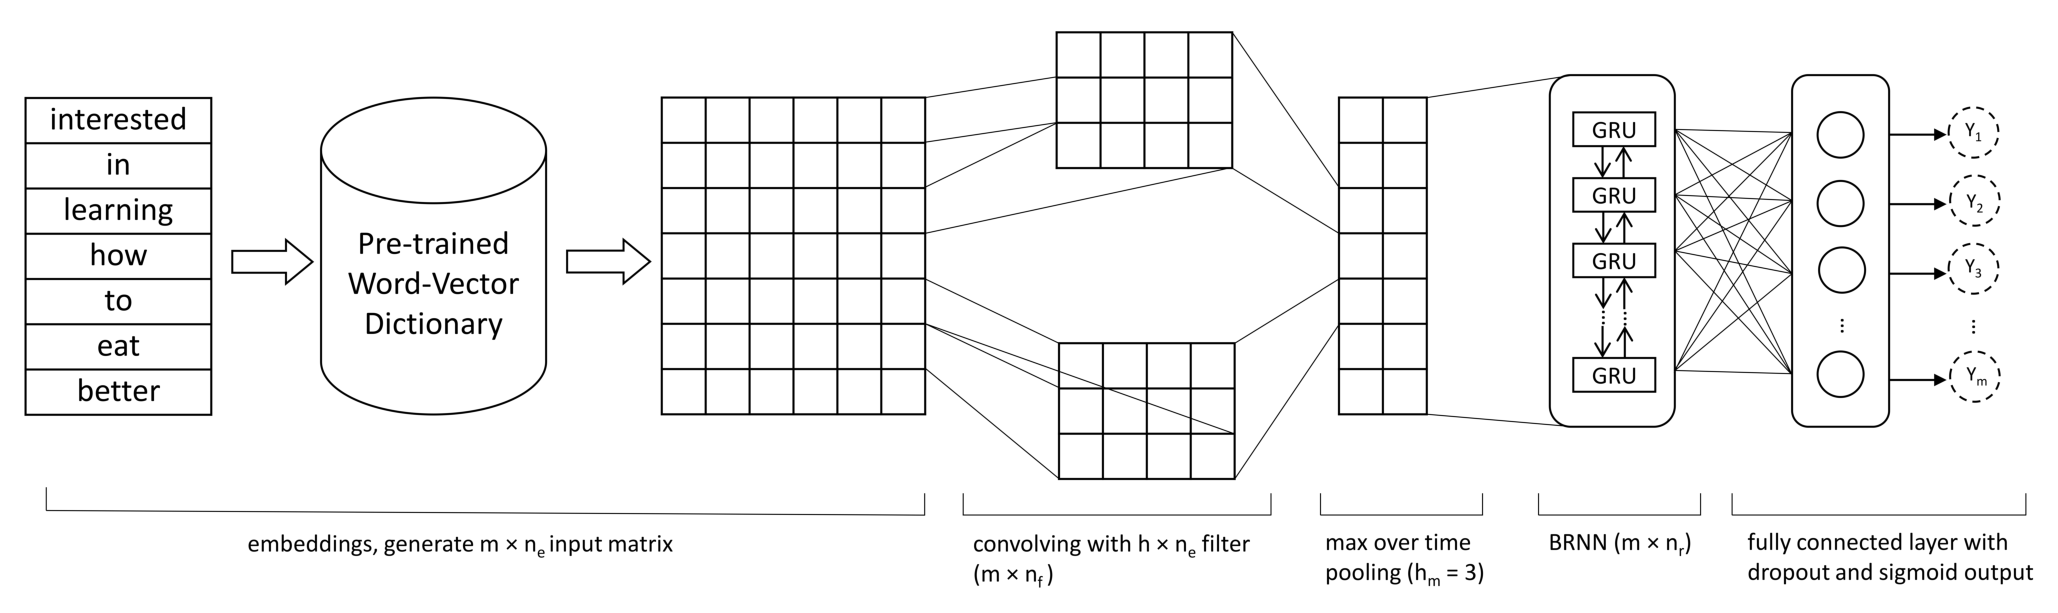
\includegraphics[width=1.0\textwidth]{figures/CRNN.eps}
    \caption{\textbf{Architecture of convolutional recurrent neural networks for automatic segmentation of e-Coaching emails}}
    \label{fig:crnn}
\end{figure}

E-coaching email exchanges are represented as a sequence of $m$ words and punctuations, which are fed into the input layer to produce a $m \times n_e$ matrix after fetching the pre-trained word vectors. When POS tags are used in combination with word embeddings, 10-dimensional POS vectors are concatenated with 300-dimensional word vectors to obtain new vectors $n_e = n_w + n_p$ of size 310. The primary purpose of convolution is to extract new features depending on neighbor words. We used 1D convolution which simply moves one step at a time on vertically. In this layer, one filter is responsible for extraction of one feature. After applying $n_f$ different filters with zero-padding on both sides of the text, $n_f$ useful features are produced in the convolution layer for each word. A max pooling operation was then performed over time to find the most significant features in a text region. The bidirectional recurrent layer receives new features extracted in the convolution layer. RNN is usually used to capture the previous history. Moreover, bidirectional RNN is capable of capturing both previous and past histories because bidirectional RNN utilized the features by looking at forward and backward states. The purpose of the fully connected layer is to use the bidirectional RNN layer output for classifying each word or punctuation into ``new segment'' and ``same segment'' classes. Since a fully connected layer has a greater number of parameters, they are more likely excessively co-adapt these parameters causing over-fitting. To prevent this over-fitting problem, dropout is used to randomly drop 50\% of the connections on the fully connected layer. After that, a sigmoid operation is performed on the output layer to provide the probability of whether the word or punctuation precedes a new segment or not. We experimentally determined the optimal parameters and found that the best performance is achieved with 5 folds cross-validation when filter length in convolution layer is 7, number of filters is 100, max-pool size is 3, convolutional layer activation is $relu$, RNN layer activation is $tanh$ and number of recurrent units in RNN is 200. Adam\cite{kingma2014adam} is used for optimization and the early stopping strategy is applied with 50 epochs when the batch size is 32 and the learning rate is 0.001. To utilize our source codes by other research studies, source codes of all experiments will be publicly available\footnote{https://github.com/teanalab/xxxxx} upon acceptance of this paper for publication.
  
\subsection*{\textit{Evaluation metrics}}
We report standard metrics for experiments (precision, recall and F1-measure) to evaluate the performance of binary classifiers.\cite{aas1999text} However, accuracy is not reported as a performance metric because accuracy is highly sensitive to the prior class probabilities and does not fully describe the actual difficulty of the decision problem for an unbalanced dataset. The results are reported based on 5 folds cross-validation and weighted macro-averaging over the folds. We also estimate the area under the receiving operating characteristics (ROC) curve\cite{kumar2011receiver} (AUC) metric due to its effectiveness in measuring the quality of binary classifiers for imbalanced datasets. \cite{hu2015kernelized}

\section*{Results}
Our experimental results have four important directions. First, the optimal dimension of word embeddings and sample size of MLP models are reported. Second, results are reported with respect to ``new segment'' class as well as weighted average over ``new segment'' and ``same segment'' classes in Table~\ref{tab:result_base}. Third, classification performance of different machine learning methods are outlined in Table~\ref{tab:result_weighted_avg} when word embeddings or lexical features are used in combination with punctuation and POS features. Fourth, the impact of the individual, as well as their combination on the segmentation task, are reported.

\begin{figure}[!htb]
    \centering
    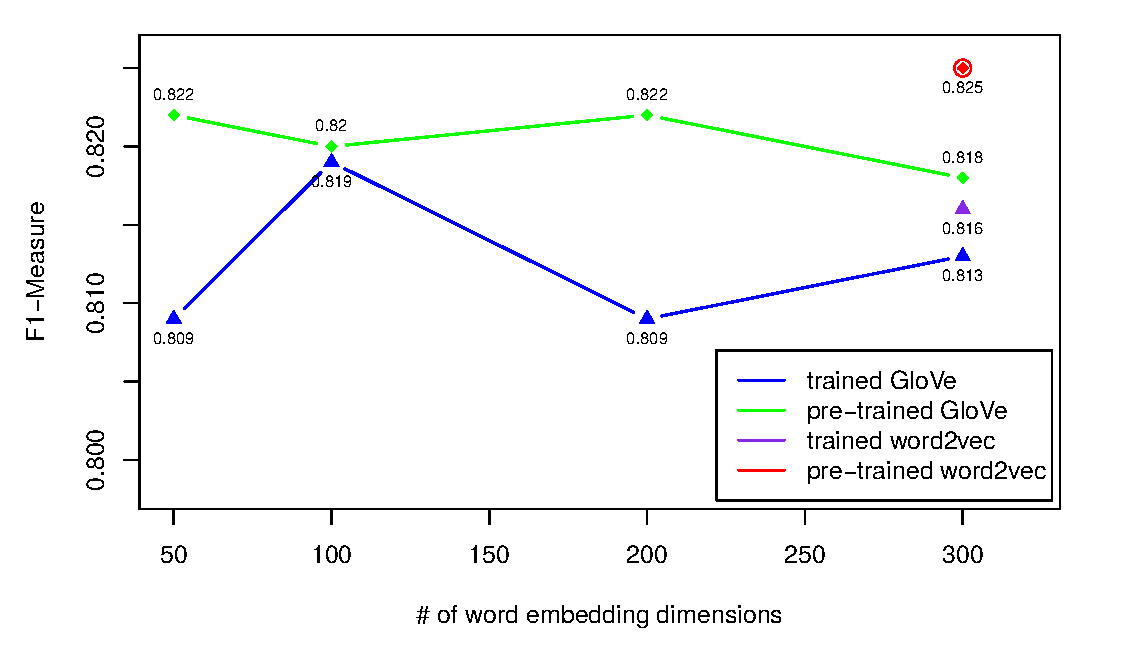
\includegraphics[width=0.5\textwidth]{figures/embedding-dimension.eps}
    \caption{\textbf{Performance of CRNN model on e-Coaching email segmentation by varying the dimension of pre-trained and trained word embeddings with GloVe and word2vec models}}
    \label{fig:embedding-dimension}
\end{figure}   
 
Figure~\ref{fig:embedding-dimension} illustrates the performance of CRNN model on e-Coaching email segmentation by varying the dimension of pre-trained and trained word embeddings with GloVe and word2vec models. It was observed that best performance achieved with pre-trained 300-dimensional word2vec word vectors when three types of features are used together. Therefore, we report our results with word2vec 300-dimensional word vectors for all deep learning models used in this study. For MLP models, the first layer input was prepared by the summation of first $l$ word vectors and last $l$ word vectors when a sample contains $2l$ words or punctuations. Figure~\ref{fig:length-mlp} demonstrates the performance of MLP model on e-Coaching email segmentation by varying the value of $l$. It was observed that the best performance of MLP is achieved when $l = 2$. Therefore, results of all MLP are reported with $l = 2$ in the remaining part of this section.    

\begin{figure}[!htb]
    \centering
    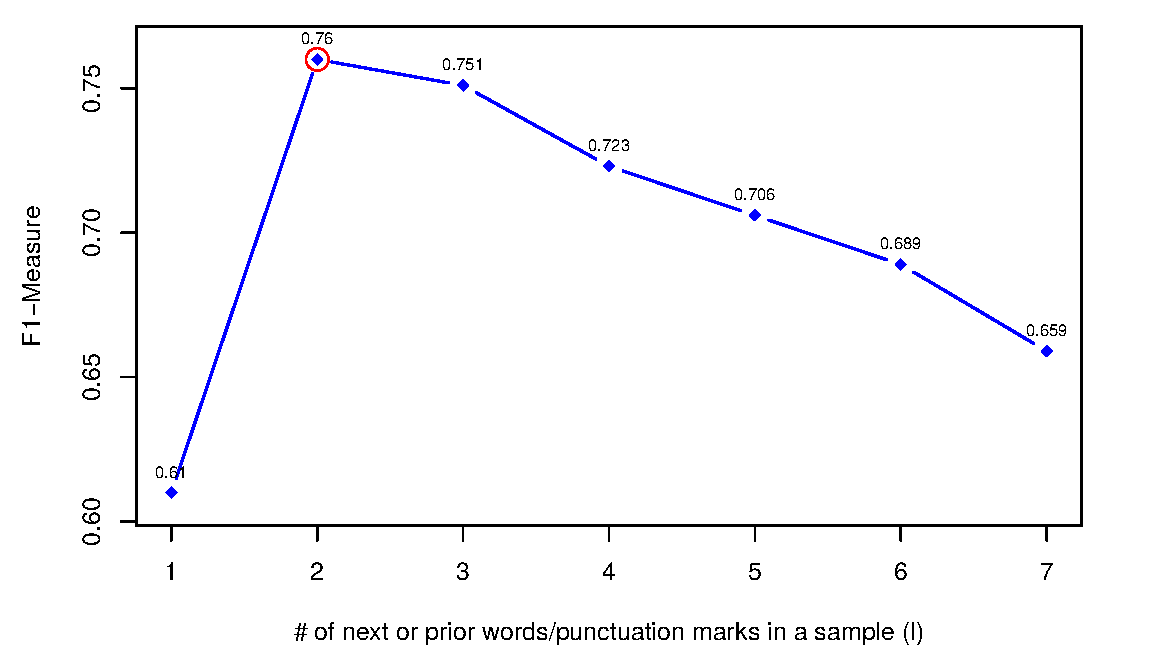
\includegraphics[width=0.5\textwidth]{figures/length-mlp.eps}
    \caption{\textbf{Performance of MLP model on e-Coaching email segmentation by varying the length of sample size}}
    \label{fig:length-mlp}
\end{figure}

As follows from Table~\ref{tab:result_base}, CRNN outperforms all other models in terms of recall and F1-measure achieving 0.797 recall with 0.785 F1-measure for new segment detection. CRNN also shows superior performance in all performance metrics for weighted average over ``new segment'' and ``same segment'' classes. BRNN demonstrates the lowest performance among all models in terms of precision and F1-Measure. On the other hand, MLP has the highest precision of 0.836 when word embeddings or lexical features are used to identify ``new segment''. CRF achieves 0.733 F1-Measure in new segment class and 0.984 F1-Measure in overall, which demonstrates the second highest performance to identify ``new segment'' as well as a weighted average over both classes. Experimental results indicate that performance of all classifiers as a weighted average over both classes is remarkably higher compared to ``new segment'' class, which is expected since 96.95\% instances belong to the ``same segment'' categories and 99.3\% of them correctly classified. For example, as a weighted average over ``new segment'' and ``same segment'' classes, CRNN achieves 27.23\%, 23.71\% and 25.61\% higher precision, recall and F1-measure, respectively, compared to ``new segment'' detection. \\

\begin{table}[ht]
\centering
\caption{\textbf{Performance of CRF, MLP, BRNN and CRNN methods for identification of ``new segment'' class as well as weighted average over ``new segment'' and ``same segment'' classes when word embeddings or lexical features are used. The highest value for each performance metric is highlighted in bold.}}
\label{tab:result_base}
  \begin{tabular}{|l|l|l|l|l|l|l|}
  \hline
   \multirow{2}{*}{\textbf{Method}} & \multicolumn{3}{|c|}{\textbf{New Segment}} & \multicolumn{3}{|c|}{\textbf{Overall}} \\\cline{2-7}
   & \textbf{Precision}  & \textbf{Recall} & \textbf{F1-Measure} & \textbf{Precision}  & \textbf{Recall} & \textbf{F1-Measure} \\ \hline    
 CRF & 0.782 & 0.691 & 0.733 & 0.983 & 0.984 & 0.984 \\ \hline
 MLP & \textbf{0.836} & 0.593 & 0.694 & 0.982 & 0.983 & 0.982 \\ \hline
 BRNN & 0.606 & 0.680 & 0.641 & 0.977 & 0.976 & 0.976 \\ \hline
 CRNN & 0.775 & \textbf{0.797} & \textbf{0.785} & \textbf{0.986} & \textbf{0.986} & \textbf{0.986} \\ \hline
  \end{tabular}
\end{table}                         


\begin{table}[ht]
\centering
\caption{\textbf{Performance of CRF, MLP, BRNN and CRNN methods for identification of ``new segment'' class as well as weighted average over ``new segment'' and ``same segment'' classes when all features are used together. The highest value for each performance metric
is highlighted in bold.}}
\label{tab:result_weighted_avg}
 \begin{tabular}{|l|l|l|l|l|l|l|}
  \hline
   \multirow{2}{*}{\textbf{Method}} & \multicolumn{3}{|c|}{\textbf{New Segment}} & \multicolumn{3}{|c|}{\textbf{Overall}} \\\cline{2-7}
   & \textbf{Precision}  & \textbf{Recall} & \textbf{F1-Measure} & \textbf{Precision}  & \textbf{Recall} & \textbf{F1-Measure} \\ \hline    
 CRF & 0.813 & 0.772 & 0.792 & 0.988 & 0.988 & 0.988 \\ \hline
 MLP & \textbf{0.817} & 0.710 & 0.760 & 0.986 & 0.987 & 0.986 \\ \hline
 BRNN & 0.683 & 0.820 & 0.745 & 0.985 & 0.983 & 0.984 \\ \hline
 CRNN & 0.789 & \textbf{0.864} & \textbf{0.825} & \textbf{0.990} & \textbf{0.989} & \textbf{0.989} \\ \hline
  \end{tabular}
\end{table}      

Table~\ref{tab:result_weighted_avg} summarizes the results of all models for segmentation of e-Coaching emails when word embeddings or lexical features are used in combination with punctuation and POS features. Similar to results in Tables~\ref{tab:result_base}, CRNN demonstrates the highest performance among all methods achieving 0.864 recall with 0.825 F1-Measure for ``new segment'' class and 0.990 precision with 0.989 recall and F1-Measure for overall. BRNN and CRF show the lowest and second highest performance, respectively, for email segmentation among all methods. We observed that classification performance significantly improved for ``new segment'' class when word embeddings or lexical features are used in combination with punctuation and POS features. Precision increases by 3.96\%, -2.27\%, 12.71\% and 1.81\%; recall increases by 11.72\%, 19.73\%, 20.59\% and 8.41\%; and F1-measure increases by 8.05\%, 9.51\%, 16.22\% and 5.1\% for CRF, MLP, BRNN and CRNN methods, respectively, in new segment detection when all features are utilized together. Similarly, precision increases by 0.51\%, 0.41\%, 0.82\% and 0.41\%; recall increases by 0.41\%, 0.41\%, 0.72\% and 0.3\%; and F1-measure increases by 0.41\%, 0.41\%, 0.82\% and 0.3\% for CRF, MLP, BRNN and CRNN methods, respectively, in weighted average over ``new segment'' and ``same segment'' classes when word embeddings or lexical features are used in combination with punctuation and POS features.\\

\begin{table}[ht]
\centering
\caption{\textbf{AUC values of all classifiers demonstrating the impact of word embeddings, punctuation and POS features on email segmentation. Highest AUC value for each feature set across all models is highlighted in boldface.}}
\label{tab:result_roc}
 \begin{tabular}{|l|l|l|l|l|}
  \hline
\multirow{2}{*}{\textbf{Features}} & \multicolumn{4}{|c|}{\textbf{AUC}} \\\cline{2-5}
 & \textbf{CRF} & \textbf{MLP}  & \textbf{BRNN} & \textbf{CRNN} \\ \hline      
 word embeddings only & \textbf{0.966} & 0.951 & 0.920 & 0.965 \\ \hline
 word embeddings + POS & \textbf{0.973} & 0.953 & 0.920 & 0.962 \\ \hline
 word embeddings + punctuation & \textbf{0.993} & 0.989 & 0.982 & 0.988 \\ \hline
 all features & \textbf{0.994} & 0.992 & 0.981 & 0.986 \\ \hline
  \end{tabular}
\end{table}      

% Baseline ROC results: BRNN: 0.9198, MLP: 0.9507, CRF: 0.9662, CRNN: 0.9648
% Proposed ROC Results: BRNN: 0.9807, MLP: 0.992, CRF: 0.9937, CRNN: 0.9859

Table~\ref{tab:result_roc} shows the impact of individual features as well as their combination on the segmentation task. Although CRF provides the second highest classification results, it shows best AUC values, achieving 0.966 AUC when only lexical features are used and 0.994 AUC when a combination of lexical, punctuation and POS features are used. Influence of the punctuation and POS features is also consistent in AUC values, which increase by 2.9\%, 4.31\%, 6.63\% and 2.18\% for CRF, MLP, BRNN and CRNN methods, respectively. Individually, POS and punctuation features improve the performance of all classifiers except CRNN when word embeddings are used with POS features. CRF and MLP achieve their highest AUCs when all features are used together. On the other hand, BRNN and CRNN demonstrate the highest AUCs when word embeddings are combined with punctuation features. 

\section*{Discussion}
This study is the first effort to evaluate the automatic segmentation of e-Coaching emails. Experimental results indicate that CRNN is the best model among all machine learning methods considered for this study. CRNN achieved 0.989 F1-measure in overall and 0.825 F1-measure for detecting ``new segment''. The robust performance of CRNN provides the evidence that deep learning models are capable to learn the hidden characteristics of MI behaviors from the clinical exchange. It also indicates that punctuation and POS features are important with word embeddings or lexical features for all machine learning methods are employed. Although the domain of this study was intentionally quite small, we believe that our study is not limited to the e-Coaching domain and it can be successfully applied to other domains, in which discourse segmentation is a preliminary step for annotation.

Punctuation mark and POS features made a significant improvement in the performance of machine learning and all deep learning methods. Specially, punctuation features have the higher individual impact on model performance compared to POS features. In all cases, every method performs better, when word embeddings or lexical features are used in combination with punctuation and POS features. This results also indicate that segmentation performance might be improved by adding additional relevant features. 

The convolutional layer made a significant difference between the performance of CRNN and BRNN on email segmentation. CRNN demonstrates 22.5\% and 10.7\% higher F1-Measure in ``new segment'' detection and 1\% and 0.5\% higher F1-Measure in overall compared to BRNN when word embeddings and all features are used, respectively. In CRNN, convolution layer performed a series of convolutions and pooling operations during which a number of high-level important features are extracted from the word embeddings of e-Coaching emails. These high-level features are then utilized by the bidirectional RNN of CRNN model, which provide an improved performance on email segmentation. On the other hand, traditional BRNN model received words as input features and their word embeddings are directly utilized in the input layer.  

\begin{figure}[!htb]
    \centering
    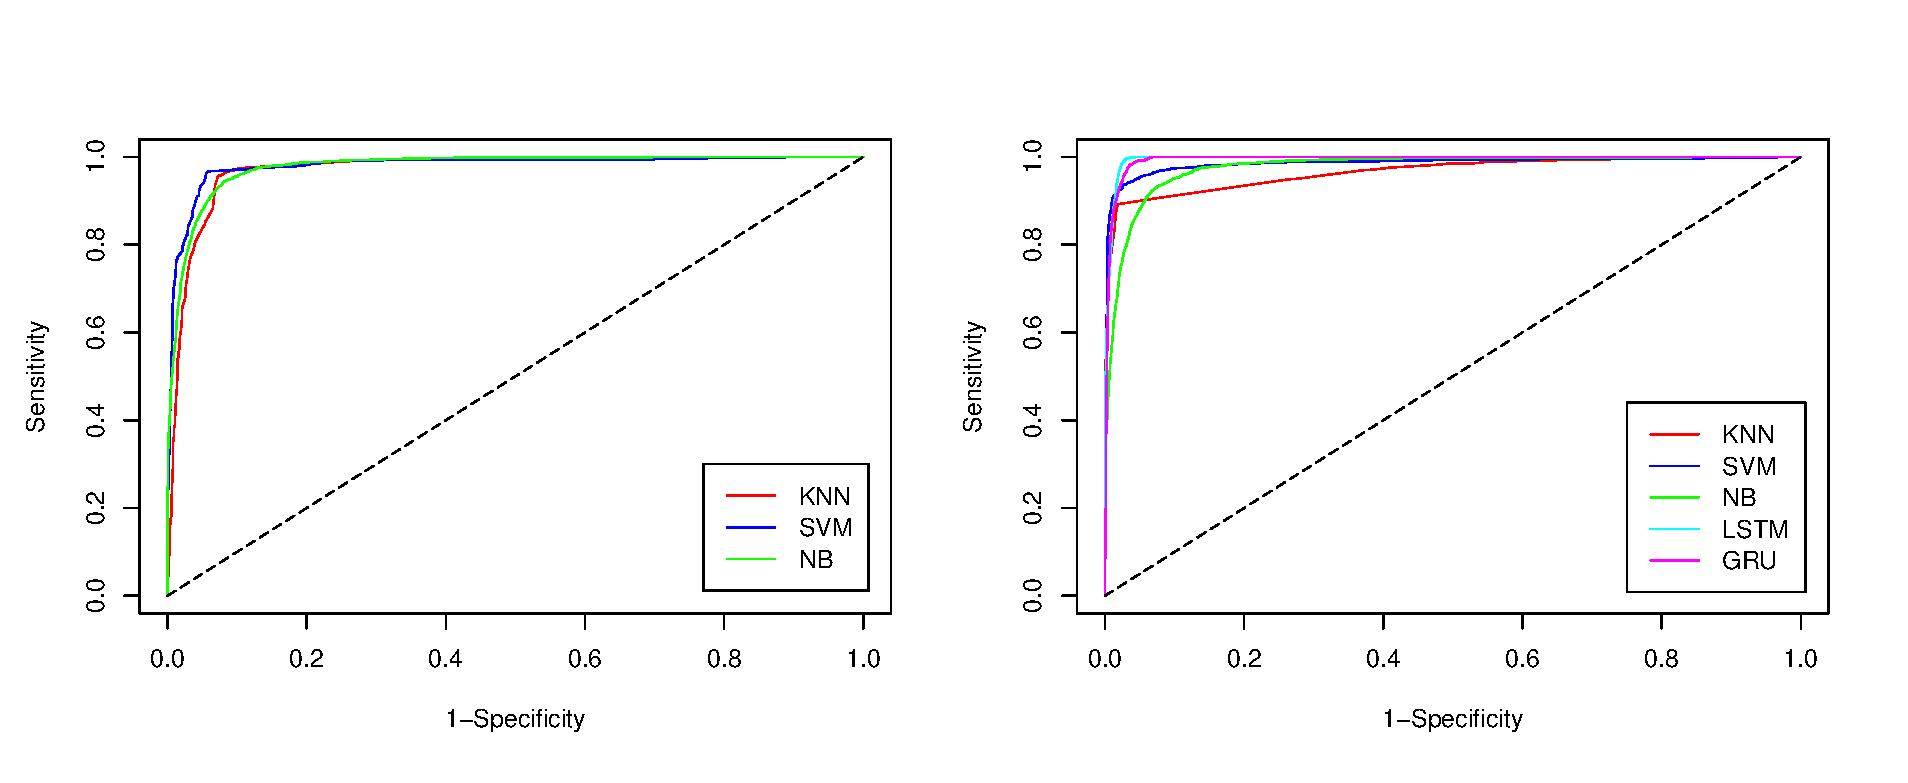
\includegraphics[width=1.0\textwidth]{figures/roc-curves.eps}
    \caption{\textbf{Receiver operating characteristic curves showing the performance of binary classifiers for the segmentation of e-Coaching text when only word embeddings or lexical features (left) and combination of word embeddings or lexical, punctuation and POS features (right) are used}}
    \label{fig:roc-curves}
\end{figure}

In this paper, results are reported by ``new segment'' class as well as weighted average over both classes to avoid confusion regarding overall model performance due to severe class imbalance. In addition, standard metrics: precision, recall and F1-measure were used to eliminate doubt about the model performance since accuracy is misleading for imbalanced datasets. AUC is also utilized due to its effectiveness in measuring the quality of binary classifiers for imbalanced datasets,\cite{hu2015kernelized} which are demonstrated by the ROC curves in Figure~\ref{fig:roc-curves}. 

Although punctuation mark plays an important role in segmentation boundary detection, a few errors were encountered by the presence of punctuation marks in boundary identification. For example, a text segment from an e-Coaching email \textit{``A typical day in regards to fruit and vegetable has me eating about a serving at breakfast (our caf has cut up fruit) and then maybe a piece of fruit later in the day or as a snack. Vegetable tends to be a side serving at lunch and dinner and I get celery or carrot cuts with dressing for a snack a lot of times. I could probably add some sort of vegetable into my breakfast (like spinach in an omelet) and snack on another piece of fruit when I am hungry rather than the junk food I tend to eat.''} incorrectly segmented after the first sentence where a punctuation mark was encountered. Similarly, additional information is a common cause for misclassification of an email segment into multiple segments. For instance, the first sentence of the above email segment represents a positive commitment to adolescent's behavior change then next two sentences provide an additional information to support their commitment. 

The limitation of this study is that e-Coaching data is collected from a single medical institute; formatting, style and email segment can be different in other settings. Therefore, there is a need to replicate the experiments with different data sets. As our future work, we plan to evaluate our approach to other datasets for discourse analysis. 
 
\section*{Conclusion}
Segmentation of e-Coaching emails is an integral part of developing e-Coaching interventions. Although several studies have focused on clinical interventions, they are limited by the qualitative coding of clinical interactions. In addition, previous studies in the medical domain mainly segmented clinical text into sections and sentences, none of them considered segmentation of text into groups of MI behaviors in the setting of discourse analysis with emails. In this paper, we compared the performance of machine learning models for the task of segmentation of e-Coaching text. We found out that CRNN provides the best performance for the segmentation of text in terms of all performance metrics. Manual segmentation of e-Coaching data is a very resource-intensive and time-consuming task, which can significantly decrease the time and effort required to develop an effective behavioral intervention. Our proposed methods can help to identify individual text segments, which can be annotated directly with a classification model. This approach will also help in developing fully automated e-Coaching and accelerate the pace of identifying effective communication strategies.

\section*{Acknowledgments}
This study was supported by a grant from the National Institutes of Health, NIDDK R21DK108071, Carcone and Kotov, MPIs. We would like to thank the research staff and student assistants in the Department of Family Medicine and Public Health Sciences at Wayne State University School of Medicine for their help in preparing the training dataset. 

\bibliographystyle{vancouver}
\bibliography{manuscript}

\end{document}
